\documentclass{article}
\usepackage[T1]{fontenc}
\usepackage{lmodern}
\usepackage{graphicx}
\usepackage{amsmath,amssymb}
\usepackage[a4paper,margin=2cm]{geometry}
\usepackage[absolute,overlay]{textpos}
\setlength{\TPHorizModule}{1mm}
\setlength{\TPVertModule}{1mm}
\usepackage[indonesian]{babel}
\usepackage{hyperref}
\setlength{\emergencystretch}{2em}
% unit: Halaman 4

\begin{document}

% === Halaman 4 (llm) ===

\begin{itemize}
    \item Ukuran blok pesan = 64 bit
    \item Panjang kunci = 256 bit
    \item Jumlah putaran = 32 putaran
    \item Setiap putaran menggunakan kunci putaran.
    \item Kunci putaran sebenarnya hanya ada 8 buah, $K_1$ sampai $K_8$, namun karena ada 32 putaran, maka 8 buah kunci putaran ini dijadwalkan penggunaannya.
\end{itemize}

\vspace{10mm}

\begin{itemize}
    \item Standard GOST yang baru menspesifikasikan \textit{cipher} blok 128-bit yang diberi nama \textit{Kuznyechik}.
\end{itemize}

% deskripsi: Tabel 6.2 Penjadwalan kunci internal GOST yang menunjukkan pemetaan antara nomor putaran (1-32) dengan kunci internal ($K_1$ sampai $K_8$)
% bbox normalisasi: [0.1080, 0.4420, 0.8570, 0.7380]
\begin{textblock*}{157.29mm}(22.68mm,131.27mm)
\noindent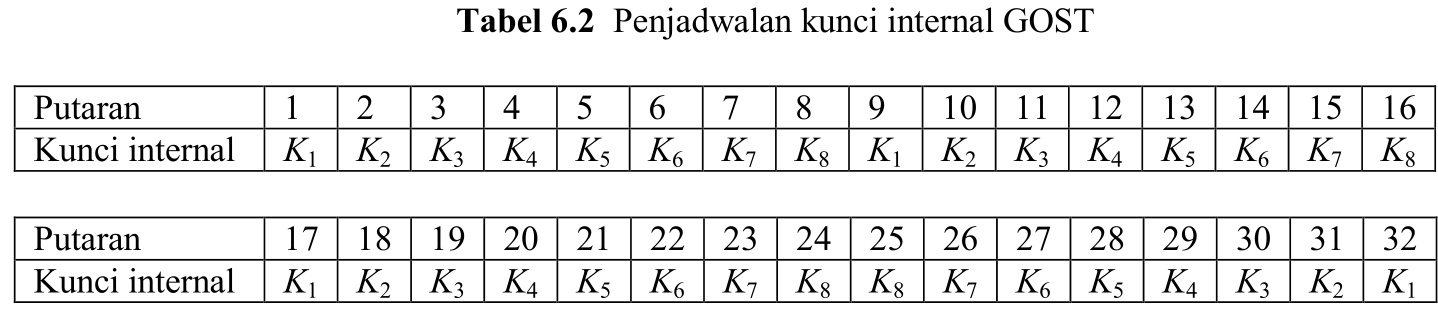
\includegraphics[width=157.29mm,height=87.91mm]{../../images/llm/page_004_img_01.png}%
\end{textblock*}

\end{document}
